\chapter{Systém PerfEval}

\section{Popis systému}

Systém PerfEval je konzolová aplikace, jejíž činnost je ovládaná příkazy a~parametry na~příkazové řádce.
Příkazy umožňují inicializovat systém, přidávat nové výsledky měření a~vyhodnocovat mezi sebou výsledky
měření dvou verzí.

\subsection{Průběh vyhodnocování}

Hlavní funkcionalitu pro~vyhodnocování poskytuje třída EvaluateCLICommand. Celý úkol vyhodnocování výkonu
byl rozdělen do~tří oddělených kroků.

Jako první dojde k~naparsování výsledků měření dvou porovnávaných verzí. Parsování probíhá pomocí
implementace rozhraní MeasurementParser, který umí naparsovat potřebný formát výsledků měření, které
se budou porovnávat. Výsledkem parsování vzniknou dvě instance třídy Samples, která reprezentuje vzorky
výsledků měření.

Následně se tyto dvě instance porovnají pomocí metody compareSets na~třídě PerformanceEvaluator. Instance třídy
PerformanceEvaluator k~porovnání dvou instancí Samples využívá implementace rozhraní StatisticTest. Konkrétně
tato implementace rozhoduje o~tom, jaký statistický test se při porovnávání vzorků použije.

Statistický test, který implememtuje rozhraní StatisticTest, musí mít metody calcCIInterval a~calcMinSampleCount.
Metoda calcCIInterval vrací intervalový odhad rozdílu náhodných veličin, které jsou reprezentovány konkrétními
naměřenými vzorky.

Pokud tento interval neobsahuje nulu, pak lze s~požadovanou přesností a~pravděpodobností usuzovat,
že rozdělení náhodných veličin jsou různá. Pokud jsou rozdělení různá, pak se jako kladný výsledek testu připouští
zlepšení výkonu, nebo pokud je nový průměr v dané toleranci.

Pokud interval obsahuje nulu, tak je vyhodnocení výsledku testu výkonu složitější. Pokud je interval spolehlivosti
dostatečně úzký, tak považujeme rozdělení náhodných veličin za stejná a~test výkonu dopadl kladně. Pokud interval
spolehlivosti není dostatečně úzký, tak test výkonu neprošel. Následně se pomocí metody calcMinSampleCount určí
kolik měření by bylo potřeba, aby byl interval spolehlivosti dostatečně úzký. Spočtený počet vzorků s~informací o~tom,
zda-li je, nebo není možné je změřit, bude přidán k~výsledkům porovnávání.

Posledním krokem při vyhodnocování je zavolání metody printResults na~implementaci rozhraní ResultPrinter. Tato metoda
vypíše instanci MeasurementComparisonResultCollection, která reprezentuje všechny výsledky jednotlivých testů výkonu.
Po~vypsání výsledků požadovaným způspobem dle dodané implementace ResultPrinter se nastaví správný exit kód. V~případě,
že všechny testy dopadly kladně, pak bude exit kód 0. V~případě, že alespoň v~jednom případě došlo ke~zhoršení, pak bude
exit kód 1. V~případě, že dojde k~nějaké výjimce, tak exit kód bude větší než 100. Touto výjimkou může být například
neexistence některého ze~souborů s~naměřenými výsledky v~důsledku jeho smazání, nebo přesunutí.

Na následujícím obrázku je k~vidění architektura části systému právě kolem třídy EvaluateCLICommand, která zajišťuje
průběh vyhodnocování testů výkonu.

    \begin{figure}[h!]
        \centering
        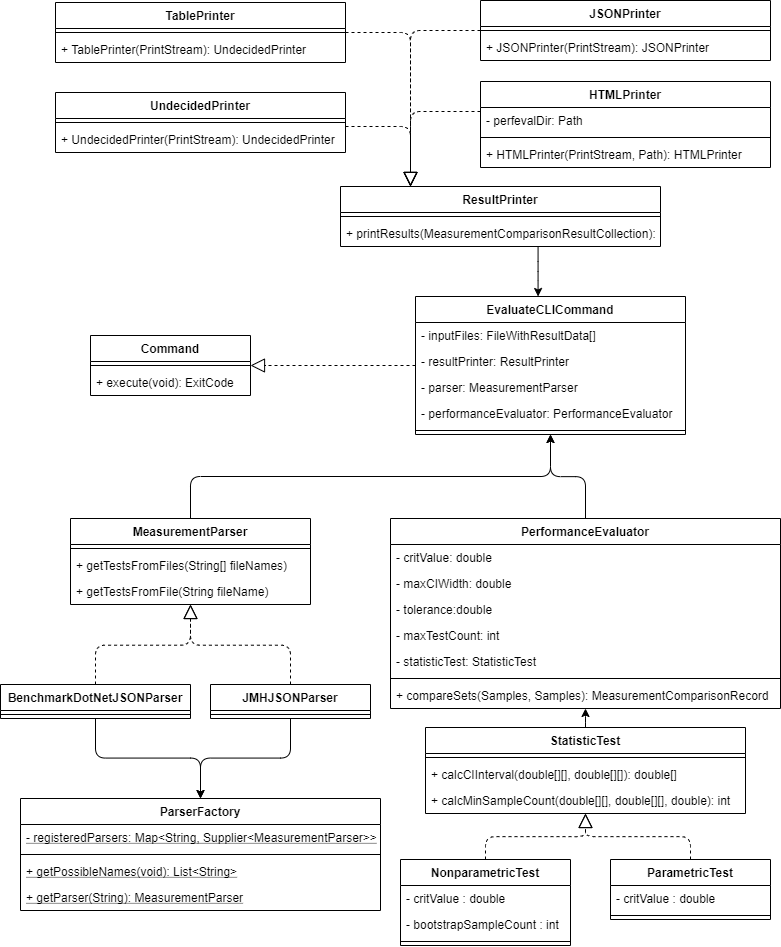
\includegraphics[width=0.9\textwidth]{../img/perfeval_evaluate.png}
        \caption{Objektový návrh časti PerfEvalu pro porovnávání výsledků měření}
    \end{figure}

Hlavní myšlenka návrhu je tok dat programem. Po~zpracování příkazové řádky dostane instance EvaluateCLICommand informace
o~soubourech se kterými bude pracovat. Při~konstrukci dostane správné implementace ResultPrinter,
MeasurementParser a~instanci třídy PerformanceEvaluator se správnou instancí StatisticTest.
Data plynou programem tak, že se naparsují pomocí implementace třídy MeasurementParser. Naparsované výsledky
se pomocí statistického testu vyhodnotí mezi sebou. Výsledky porovnání se vypíšou pomocí implementace rozhraní
ResultPrinter.

\subsection{Inicializace systému PerfEval}

Před použitím systému PerfEval k~vyhodnocování je nutné jej inicializovat. Inicializace umí rozpoznat zda-li se nachází
v~kořenovém adresáři Git repozitáře. Rozpoznávání probíhá tak, že se hledá soubor s názvem .git.

Inicializace probíhá tak, že se zjistí přítomnost .git souboru. Z~příkazové řádky se zjistí jaký parser (implementace
třídy MeasurementParser) pro~naměřené hodnoty se bude používat. Vyrobí výchozí konfigurace. Do~výchozí konfigurace
se dodají informace o~git repozitáři a~o~parseru. Nakonec se vyrobí složka se v adresáři, kde uživatel program spustil
vyrobí složka .performance a~v~ní soubory .gitignore a~config.ini. Soubor config.ini obsahuje konfiguraci systému PerfEval
pro~jeden projekt jehož výkon mezi verzemi se bude porovnávat.

\begin{figure}[h!]
    \centering
    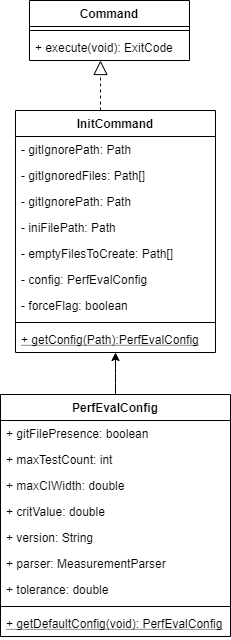
\includegraphics[height=0.5\textheight]{../img/perfeval_init.png}
    \caption{Objektový návrh časti PerfEvalu pro inicializaci}
\end{figure}

Z~obrázku je patrné, že třída InitCommand úzce spolupracuje s~třídou PerfEvalConfig. Třída PerfEvalConfig reprezentuje
obsah souboru config.ini. Provedení metody execute na~třídě InitCommand provede inicializaci systému PerfEval výše
zmíněným způsobem.

\subsection{Přidávání nových výsledků testů}

Uživatel musí každý výsledek měření výkonu zaznamenat do~systému PerfEval. Pokud výsledek měření zaznamenán, nebude s~ním
PerfEval vůbec pracovat. Přidávat je možné soubory samostatně, nebo z~adresáře. Při~přidávání souborů z~adresáře budou
přidány všechny soubory a~to i~soubory zanořené ve~vnitřních adresářích zadaného adresáře.

\begin{figure}[h!]
    \centering
    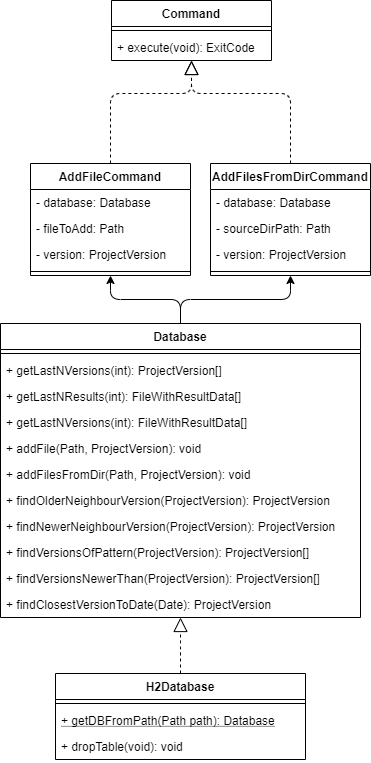
\includegraphics[height=0.5\textheight]{../img/perfeval_h2db.png}
    \caption{Objektový návrh časti PerfEvalu pro přidávání výsledků měření}
\end{figure}

Na obrázku je vidět, že za~oběma příkazy pro přidávání výsledků měření stojí jedna implementace rozhraní Database.
Jediná existující implementace tohoto rozhraní využívá technologie H2 databáze. Jedná se o~technologii, která umožňuje
vést si databázi lokálně v~rámci souboru a~pokládat na ní klasické SQL dotazy.

Implementace rozhraní Database pomocí technologie H2 je třída H2Database. V~rámci databáze pro jeden projekt, který
PerfEval spravuje jsou lokální soubory pro H2 databázi uloženy v adresáři .performance. Databáze pro správu dat o~výsledcích
měření má jen jednu tabulku. V~této tabulce jsou informace o~cestě k~souboru a~informace o~verzi.

\section{Rozbor alternativ v řešení}
Při~vývoji systému PerfEval došlo k~několika rozhodnutím, které výrazně ovlivnily jeho fungování a~architekturu.
Nejdůležitější rozhodnutí, která byla v~průběhu výoje provedena jsou v~následujících částech podrobně vysvětleny.

\subsection{Grafické rozhraní}
PerfEval je aplikace používaná z příkazové řádky. Od~počátku plánování bylo zamýšlené, že~se bude
ovládat pomocí příkazové řádky. Je určen pro porovnávání výsledků testování výkonu dvou verzí softwaru.
Pomocí exit kódu signalizuje, zda-li nedošlo ke~zhoršení výkonu.

PerfEval měl mít ale i~grafickou část. V~grafické části by si mohl uživatel prohlížet dlouhodobý vývoj
výkonu jeho testovaného softwaru. K~dispozici by mu v~rámci tohoto rozhraní mělo být porovnání více verzí
v~podobě grafů. Zároveň by si uživatel mohl omezovat zobrazovaná období pro detailnější zkoumání.

Protože základní aplikace bez grafického rozhraní byla složitější než zpočátku zdálo, tak grafické
rozhraní aplikace nebylo realizováno.

\subsection{Spouštění testů systémem PerfEval}
V~počátku vývoje bylo nutné se~rozhodnout jakým způsobem bude systém přijímat a~zpracovávat výsledky testů.
V~úvahu přicházela varianta, že~uživatel provede měření výkonu sám, a~druhá varianta, že~uživatel systému
vysvětlí jakým způsobem se~testování výkonu spouští. Pokud by byla zvolena varianta, kdy PerfEval spouští testy
sám, tak by bylo nutné nalézt dostatečně univerzální způsob spouštění testů.

Aplikace a~benchmarky pro měření výkonu mohou být jak konzolové, tak grafické aplikace. Pokud by PerfEval měl
měření provádět sám, tak by téměř určitě nebyl schopen pracovat s~grafickými aplikacemi, ale byl by schopen
spouštět programy s~parametry na~příkazové řádce.

Dále by bylo nutné vysvětlit jak vypadá výstup spouštěných testů. Když pomineme formát, tak je nutné zjistit,
kam program, který provádí měření výsledky ukládá. Benchmarkovací systém BenchmarkDotNet například vypisuje
výsledky měření v podobě tabulky na standardní výstup a~zároveň ukládá strojově čitelné výsledky do~speciálního
k~tomu určeného adresáře.

Nakonec by to vypadalo tak, že při inicializaci systému uživatel zadá jak spustit test výkonu a~kam se uloží výsledek.
Tímto způsobem by došlo k~tomu, že~PerfEval by začal určovat, jak mají vypadat programy jejichž výstupy přijímá.
Na druhou stranu použití stávajícího řešení tyto nevýhody nemá. Jediné, co~musí uživatel zajistit je, že~jeho
způsob měření zvládne uložit výsledek do~souboru, který PerfEval umí zpracovat.

Stávající řešení je tedy složitější v tom, že~uživatel musí testování výkonu spouštět sám. Poté, co~spustí testování
výkonu a~dostane soubor s~výsledky je přidá do databáze výsledků systému PerfEval a~poté spustí PerfEval s~příkazem evaluate
pro porovnání výsledků testování výkonu. Kdyby se použila varianta s~tím, že si PerfEval spouští testy sám, tak
by uživatel testování a~porovnání výkonu zvládl jedním spuštěním aplikace.

\subsection{Použité statistické metody}
Pro porovnání dvou výsledků měření se používají statistické metody. Statistické metody se používají ke zjištění,
jestli výsledky měření považované za~náhodné veličiny mají stejné rozdělení, popřípadě jestli je vzorků dostatečné množství.
V~systému PerfEval jsou implementovány statistické metody bootstrap a~T-test.

Pomocí bootstrapu dochází k~iluzi, že vzorků je mnohem více, než je jich ve skutečnosti změřeno. Protože měření vzorků
je samo o~sobě dlouhotrvající proces, tak se použití této statistické metody vyplatí. Bootstrap má ale tu nevýhodu, že jeho výpočet
může oproti prostému zkoumání vzorků trvat delší dobu.

T-test je tedy možné zvolit namísto bootstrapu kvůli tomu, že je rychlejší. Oproti náhodnému vybírání vzorků z~dvoudimenzionální sady
dat, kterým vzorky odpovídají, dochází k~pouhému dosazení hodnot do vzorce.

Uživatel by se tedy při volbě testu měl rozhodovat na základě toho kolik má změřených vzorků a~kolik má času na porovnání
výsledků měření. Pokud má uživatel naměřených vzorků málo a větší množství času k vyhodnocení doporučuje se použít bootstrap.
Pokud má uživatel větší množství vzorků a~málo času je pro něho lepší použít T-test.

\subsection{Forma ukládání informací o měřeních}
Systém, který provnává výsledky měření, by měl mít nějaké informace o~tom, k~jaké verzi se měření vztahuje, nebo kde
se soubor s~výsledky nachází. Proto bylo při výovji nutné se zamyslet nad tím jakými způsoby lze tyto informace získat.
Systém PerfEval potřebuje o~výsledcích měření vědět, kde jsou uloženy a~ke~které verzi softwaru bylo měření provedeno.

První zvažovaná varianta byla, že by existovala složka do~které by uživatel vkládal výsledky měření do~adresáře určeného
systémem PerfEval, nebo do~adresáře zadaného při inicializaci systému. Po~každém měření by tedy uživatel výsledek akorát
vložil do~správné složky a~o~nic víc by se nemusel starat.

Toto řešení má několik nevýhod. Omezuje uživatele v~tom, jak musí výsledky testů ukládat. Dále by se špatně určovalo ke~
které verzi bylo měření provedeno, protože toto se ve~výsledcích měření běžnými frameworky neudává. Pravděpodobně by proto
vznikla hierarchie v tomto adresáři a~uživatel by například pomocí pojmenovávání složek určoval ke~které verzi se měření vztahuje.

Celkově tedy tento způsob poskytuje jednoduché zjištění, kde se výsledek testu nachází. Je to pevně dané. Není ale možné jednoduše
zjistit verzi, protože je nutné projít adresářovou strukturu, což může být při velkém množství dat pomalé.

Druhá zvažovaná varianta byla taková, že by PerfEval znal celý obsah souborů s~výsledky testování. Konkrétně by v~nějakém
svém adresáři měl uložený celý výstup měření ve~svém vlastním formátu, dooplněné o~vlastní poteřbná metadata. Při~zaznamenání
nových výsledků by tedy došlo k načtení celého souboru s~výsledky jeho přepracování do~formátu, kterému by PerfEval rozumněl,
a~znovuuložení do svého adresáře s~výsledky měření.

V~rámci tohoto řešení je jednoduché zjistit k~jaké verzi výsledky měření patří i~kde je soubor uložen. Místo uložení souboru
je pevně dané jako u~prvního způsobu a~verze je udaná v~metadatech uložených přímo mezi předzpracovanými výsledky. Opět
ale dochází k~prohledávání souborů na~disku jako u~první varianty. Aby byl nalezen výsledek měření pro požadovanou verzi bylo
by nutné nalézt soubor s~výsledky měření k~této verzi mezi všemi výsledky měření, které systém eviduje. Lze docílit částečného
zrychlení, pokud by se tento systém ukládánní doplnil o~nějakou variantu cache. Nicméně při testování dvou verzí z~nichž
jedna není uložena v~cache by došlo k~pomalému prohledávání celé struktury.

Tento způsob tedy Nakonec také nebyl použit, z~důvodu pomalého procházení dat uložených v~pevné paměti.

Poslední uvažované řešení je strukturované ukládání metadat o~výsledcích měření. Využije se databáze o~jedné tabulce, kde
je uvedena cesta k~výsledku měření a~verze ke které byl výsledek změřen. Uživatel do~systému nahlásí, že má nový výsledek
měření, kde je uložen, a~k~jaké verzi softwaru je měření provedeno. Systém si tato data pouze poznamená do~databáze. Při
vyhodnocení pak pomocí databázových dotazů nalezen snadno všechny soubory s~výsledky měření k~potřebné verzi.

Toto řešení poskytuje jak rychlé vkládání nových výsledků, tak rychlé vyhledávání výsledků měření k~dané verzi. Zároveň
není nutné žádné předzpracování souborů, a~tudíž není třeba je při vkládání číst.